\documentclass[12pt, a4paper]{article}

% ====== PAQUETES BÁSICOS ======
\usepackage[spanish]{babel}
\usepackage[utf8]{inputenc}
\usepackage[T1]{fontenc}
\usepackage{amsmath, amssymb, graphicx, geometry}
\geometry{margin=2.5cm}
\usepackage{fancyhdr}

% ====== ENCABEZADO ======
\pagestyle{fancy}
\fancyhf{}
\lhead{Guía de Ejercicios 4 (Resuelta)}
\rhead{Juan Ignacio Elosegui}
\cfoot{\thepage}

\begin{document}
    \section*{Ejercicio 1}
        \noindent El algoritmo de \textit{backpropagation} cumple con las siguientes opciones:
        \begin{itemize}
           \item Es un método de regularización para redes neuronales.
           \item Es un algoritmo para el cálculo del gradiente de una función.
        \end{itemize}
    \section*{Ejercicio 2}
        \subsection*{Inciso a)}
            \noindent PyTorch permite diferenciar funciones por medio de \textbf{diferenciación automática}, con el método \textit{torch.autograd}.
        \subsection*{Inciso b)}
            \noindent PyTorch permite:
            \begin{enumerate}
                \item Paralelizar operaciones en múltiples procesadores de CPU y GPU.
                    \subitem \noindent Se llama paralelismo de datos. Distribuye el trabajo computacional.
            \end{enumerate}
    \section*{Ejercicio 3}
        \noindent Sea la función \[ f(w, x, y, z) = -\left(\max(z, 2x) + 2(wy)\right) \tag{1} \] evaluada en el punto \(w = 3, x = 2, y = 4, z = 1\), y la función \[ g(w, x, y, z) = -3((4xy)+\max(w, z)) \tag{2} \] evaluada en el punto \(w = 3, x = 5, y = 2, z = 4\).
        \subsection*{Inciso 1}
            \begin{center}
                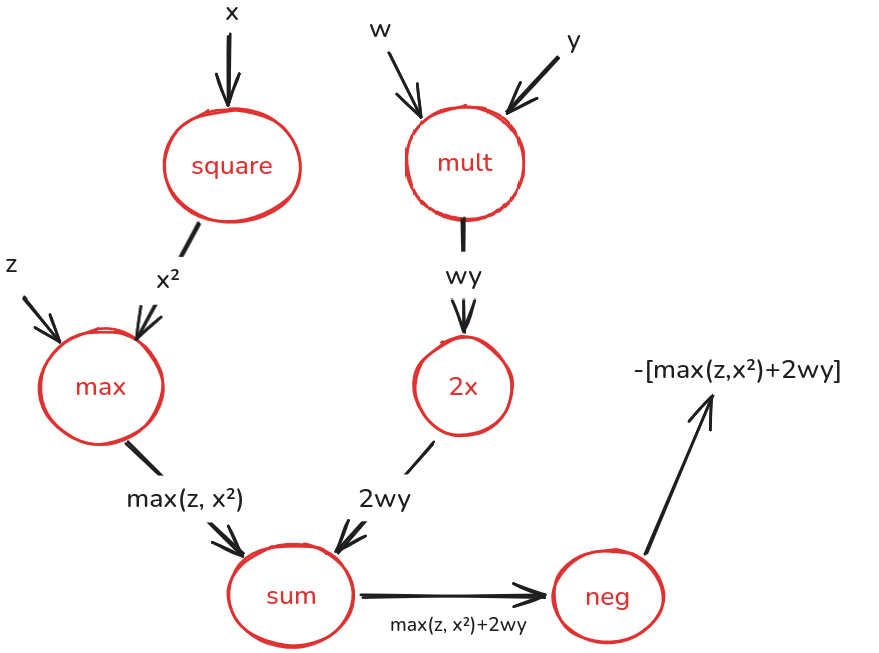
\includegraphics[width=0.7\linewidth]{figs/3.1.png}
                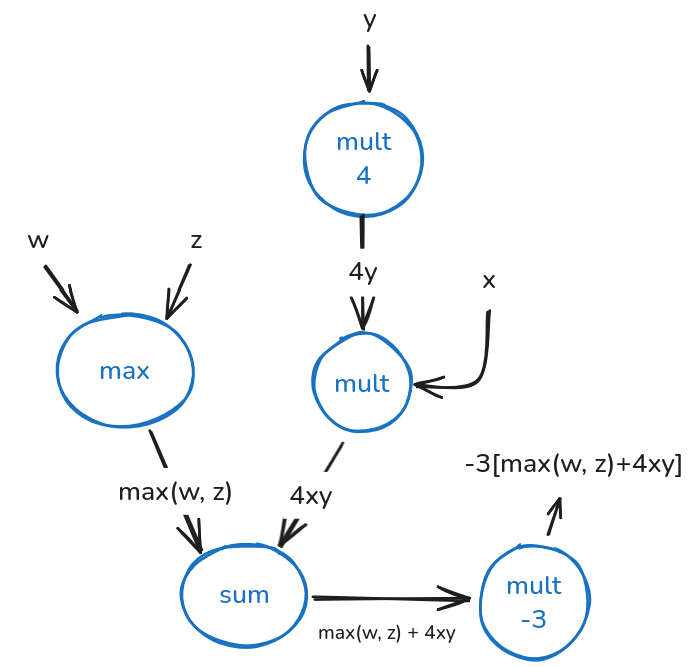
\includegraphics[width=0.7\linewidth]{figs/3.1b.png}
            \end{center}
        \subsection*{Inciso 2}
        \subsection*{Inciso 3}
    \section*{Ejercicio 4}
        \subsection*{Inciso 1}
            \[ \delta^L_j = (a^L_j - y^L_j)\,\sigma'(z^L_j) \]

            \noindent Demostración: \[ C_j = \frac12(y^L_j - a^L_j)^2 \] \[ \frac{\partial C}{\partial a^L_j} = \frac{\partial}{\partial a^L_j} \left[\frac{1}{2}(y^L_j - a^L_j)^2 \right] = (a^L_j - y^L_j) \]

            \noindent Como \(a^L_j = \sigma(z^L_j)\), entonces \[ \frac{\partial a^L_j}{\partial z^L_j} = \sigma'(z^L_j) \]

            \noindent Aplicando la regla de la cadena: \[ \delta^L_j = \frac{\partial C}{\partial z^L_j} = \frac{\partial C}{\partial a^L_j} \cdot \frac{\partial a^L_j}{\partial z^L_j} = (a^L_j - y^L_j)\,\sigma'(z^L_j) \]
        \subsection*{Inciso 2}
            \[ \delta^l_j = \sigma'(z^l_j) \sum_k \delta^{l+1}_k\, w^{\,l+1}_{jk} \]

            \noindent Usamos la igualdad de la guía: \[ \delta^l_j = \sum_k \frac{\partial C}{\partial z^{l+1}_k}\, \frac{\partial z^{l+1}_k}{\partial z^l_j} \]

            \noindent Por definición: \[ z^{l+1}_k = \sum_j w^{\,l+1}_{jk}\, a^l_j + b^{l+1}_k = \sum_j w^{\,l+1}_{jk}\, \sigma(z^l_j) + b^{l+1}_k \]

            \noindent Por lo tanto: \[ \frac{\partial z^{l+1}_k}{\partial z^l_j} = w^{\,l+1}_{jk}\,\sigma'(z^l_j) \]

            \noindent Entonces: \[ \delta^l_j = \sum_k \delta^{l+1}_k \cdot w^{\,l+1}_{jk}\, \sigma'(z^l_j) \]

            \noindent Factorizando: \[ \delta^l_j = \sigma'(z^l_j) \sum_k \delta^{l+1}_k w^{\,l+1}_{jk} \]
        \subsection*{Inciso 3}
            \[ \frac{\partial C}{\partial w^{\,l}_{ij}} = \delta^l_j\, a^{\,l-1}_i \]
            
            \noindent Demostración: Como \[ z^l_j = \sum_i w^{\,l}_{ij} a^{\,l-1}_i + b^l_j, \]

            \noindent entonces: \[ \frac{\partial z^l_j}{\partial w^{\,l}_{ij}} = a^{\,l-1}_i \]

            \noindent Usando la regla de la cadena: \[ \frac{\partial C}{\partial w^{\,l}_{ij}} = \frac{\partial C}{\partial z^l_j} \cdot \frac{\partial z^l_j}{\partial w^{\,l}_{ij}} = \delta^l_j\, a^{\,l-1}_i \]
        \subsection*{Inciso 4}
            \[ \frac{\partial C}{\partial b^l_j} = \delta^l_j \]

            \noindent Como: \[ z^l_j = \sum_i w^{\,l}_{ij} a^{\,l-1}_i + b^l_j, \] 

            \noindent entonces: \[ \frac{\partial z^l_j}{\partial b^l_j} = 1 \]

            \noindent Por lo tanto: \[ \frac{\partial C}{\partial b^l_j} = \frac{\partial C}{\partial z^l_j} \cdot 1 = \delta^l_j \]
        \subsection*{Interpretación de los $\delta$}
            Los valores $\delta^{l}_{j}$ representan el \emph{error} que la neurona $j$ de la capa $l$ contribuye al costo total. Cada $\delta$ mide cuán sensible es el costo ante un cambio en $z^{l}_{j}$, permitiendo así propagar el error hacia atrás durante el algoritmo de backpropagation.
\end{document}
